\chapter{Introduction}
\label{chp:introduction}
Nowadays, 19\% of the global energy consumption is used for lighting. For this reason, saving energy in lighting is vital. A simple way to save energy is to “simply” turn the lights off, or reduce the amount of light used when nobody is around. This thesis proposes a new method for luminaires to detect the presence of humans and objects.

The idea of human sensing is not new. Everybody in the western world has walked into a room where the lights suddenly turned on once they entered. The most common method to create this effect is to make use of a PIR (passive-infrared) sensor. By monitoring the infra-red radiation (heat) in the area, it can detect changes in the environment and toggle the light based on these changes. This method works very well but has several drawbacks. The first is that it's unable to detect objects with the same surface temperature as the environment, like for example a car where the engine has just been turned on. Another drawback is that the PIR method has no potential for communication without the addition of extra components. The new method attempts to overcome these drawbacks by only using a photo diode and the light in the visible spectrum a luminaire normally emits.

This thesis explores the idea of detecting changes in the environment with reflections of visible light. The proposed system works in the following manner: If nothing is in the area, the light will be turned on and the luminaire will illuminate the surrounding area. Some of the light will reflect off the environment back to the light source. This light can be measured with the photo diode. The signal received is a measure of the illuminated area. If something where to change in that area, a car drives by for example, then the reflections in the environment will change and therefore the light perceived by the photo diode will change as well. These changes will then result in a detection by the system. An overview of the scenario can be seen in \ref{fig:Introduction}.

This method by itself does not save energy as the light used in the system is always turned on. If we are able reduce the light output while maintaining the ability to pick up meaningful reflections, then the system would save energy. For this application we can’t simply lower the light output by reducing the current flowing into the light (analog dimming). If we for example reduce the current flowing into the light by a factor 2, then the reflections will also become twice as weak, which results in a smaller signal to detect. Another method to reduce the total light output is to decrease the amount of time the current is allowed to flow into the light (digital dimming). By turning the light on and off at a rapidly we can reduce the light output. Then, if we then measure the reflections only when the light is fully turned on, we can capture a reflection without losing signal strength.


\begin{figure}[h]
	\centering     %%% not \center
	\label{fig:Introduction}
	\subfigure[raw data received by WIFI reciever-transmitter pairs.]{\label{fig:Mov_var_a}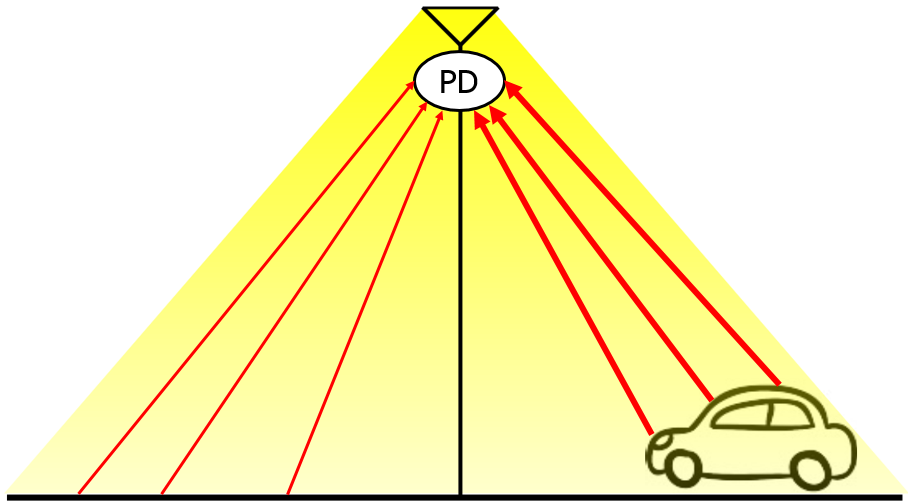
\includegraphics[width=60mm]{pics/SystemIdea.png}}
	\subfigure[Moving variance applied to the raw data.]{\label{fig:Mov_var_b}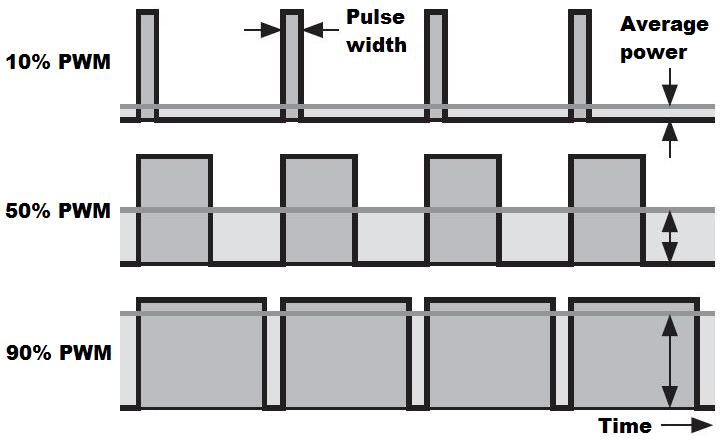
\includegraphics[width=60mm]{pics/PWM.png}}
	\caption{Analogue VS digital dimming.}
\end{figure}

\section{Problem statement}
\label{Problem statement}
Is it possible to create a system, that can detect the activity of humans or objects by measuring reflections of visible light while being invisible to the human eye?
\begin{itemize}\itemsep2pt
	\item How strong is a reflection obtained from a flash in a realistic scenario and how much does this reflection vary if a human is in the area?
	\item What are the challenges in obtaining reflections when the light is turned on for a very short time and how can they be tackled?
	\item What additional signals are received by the system (beside the reflection of the flash) and what algorithm can be used to convert the received signal in a reliable logical signal: Detection or no detection?
\end{itemize}

\section{Contributions}
\label{sec:Contributions}
This thesis proposes \textbf{Dark Sensing}, a system that uses reflections of a LED controlled with a low duty cycle (1.4\%), and therefore nearly invisible to the human eye, to detect changes in the surrounding area without active involvement of the environment.
\begin{itemize}\itemsep2pt
	\item A model, estimating the change in signal (reflected light) when a object moves under, leaves or passes by the LED in different environments.
	\item A method to convert a captured reflection of the LED into a usable measure of the environment.
	\item An algorithm which analyses features of consecutive flashes which is capable of detecting objects moving under, leaving or passing through the illuminated area.
	\item A prototype capable of detecting 99\% of all humans passing by in a realistic environment and therefore saving 98.6\% of the light used in comparison to the original situation.
\end{itemize}

\section{Organization}
\label{sec:Organization}
The thesis starts with providing background knowledge required to understand the thesis followed by an overview of the related work. It then shows that the proposed system could work with the help of a model. 